\documentclass[12pt]{exam}
\usepackage{amsthm}
\usepackage{libertine}
\usepackage[utf8]{inputenc}
\usepackage[margin=1in]{geometry}
\usepackage{amsmath,amssymb}
\usepackage{multicol}
\usepackage[shortlabels]{enumitem}
\usepackage{siunitx}
\usepackage{cancel}
\usepackage{graphicx}
\usepackage{pgfplots}
\usepackage{listings}
\usepackage{blindtext}
\usepackage{hyperref}
\usepackage{xcolor}

\definecolor{codegreen}{rgb}{0,0.6,0}
\definecolor{codegray}{rgb}{0.5,0.5,0.5}
\definecolor{codepurple}{rgb}{0.58,0,0.82}
\definecolor{backcolour}{rgb}{0.95,0.95,0.92}

\lstdefinestyle{mystyle}{
  backgroundcolor=\color{backcolour},   
  commentstyle=\color{codegreen},
  keywordstyle=\color{magenta},
  numberstyle=\tiny\color{codegray},
  stringstyle=\color{codepurple},
  basicstyle=\ttfamily\footnotesize,
  breakatwhitespace=false,         
  breaklines=true,                 
  captionpos=b,                    
  keepspaces=true,                 
  numbers=left,                    
  numbersep=5pt,                  
  showspaces=false,                
  showstringspaces=false,
  showtabs=false,                  
  tabsize=2
}

%\lstset{style=mystyle}
\usepackage{tikz}


\pgfplotsset{width=10cm,compat=1.9}
\usepgfplotslibrary{external}
\tikzexternalize

\newcommand{\class}{Laboratorio Intermedio} % This is the name of the course 
\newcommand{\examnum}{Tarea Estadistica} % This is the name of the assignment
\newcommand{\examdate}{\today} % This is the due date
\newcommand{\timelimit}{}





\begin{document}
\pagestyle{plain}
\thispagestyle{empty}

\noindent
\begin{tabular*}{\textwidth}{l @{\extracolsep{\fill}} r @{\extracolsep{6pt}} l}
  \textbf{\class} & \textbf{Name:} & \textit{Sergio Montoya Ramirez}\\ %Your name here instead, obviously 
  \textbf{\examnum} && \textit{Angelica Lopez Duarte}\\
  \textbf{\examdate} &&
\end{tabular*}\\
\rule[2ex]{\textwidth}{2pt}
% ---

\section*{Nota}

Durante el transcurso de este trabajo se hara uso de varios scripts en python (Particularmente para usar sympy que opinamos que es una de las maravillas del mundo moderno). Se pondra aqui el codigo utilizado sin embargo recomendamos fervientemente que lo mire en el repo de github: \url{https://github.com/demon-s1e7j/Universidad/tree/main/Semestre_10/LabIntermedio/Tareas/Tarea2/code}. Este ya esta comodamente organizado para tener un proyecto de uv con el que manejar los requerimientos. Eh de confesar que no estan pensados para que alguien mas los ejecute y entienda lo que retorna pero creo que sigue siendo mucho mejor que simplemente quedarse con la implementacion mostrada en este documento.

\section{Punto 2.1}

Podemos usar el codigo

\lstinputlisting[language=Python]{./code/punto_2_1.py}

lo que nos da:
\begin{lstlisting}[language=Bash]
$ uv run punto_2_1.py
promedio=26.0625
desviacion_rar=0.29166666666666663
desviacion_2_3=0.49280538030458104
error_rar=0.10311973892303816
error_2_3=0.17423301310929235
\end{lstlisting}

\section{Punto 2.6}
\subsection{}

Numero de datos: 5

\begin{itemize}
  \item $\alpha = 0.01913 \approx 0.019$
  \item $\bar{\delta} = 3.27346 \approx 3.273$
\end{itemize}


\textbf{Resultado: }$3.273 \pm 0.019$

\subsection{}

Numero de datos: 50

\begin{itemize}
  \item $\alpha = 0.002506 \approx 0.0025$
  \item $\bar{\delta} = 3.26513 \approx 3.2651$
\end{itemize}


\textbf{Resultado: }$3.25513 \pm 0.019$

\subsection{}

Numero de datos: 500

\begin{itemize}
  \item $\alpha = 0.000270 \approx 0.000270$
  \item $\bar{\delta} = 3.26681 \approx 3.26681$
\end{itemize}


\textbf{Resultado: }$3.273 \pm 0.019$

\section{Punto 3.4}

Podemos crear la funcion (sin integrarla) en sympy como
$$\frac{\sqrt{2} e^{- \frac{\left(- \mu + x\right)^{2}}{2 \sigma^{2}}}}{2 \sqrt{\pi} \sigma}$$

y con eso podemos implementar un codigo:

\lstinputlisting[language=Python]{./code/punto_3_2.py}

Que nos da como resultado:

\begin{tabular}{lll}
  \hline
  Centrado en media   & Medidas dentro del rango   & Medidas fuera del rango   \\
  \hline
  $\pm 1 \sigma$        & 68.27\%                     & 31.73\%                    \\
  $\pm 1.65 \sigma$     & 90.11\%                     & 9.89\%                     \\
  $\pm 2 \sigma$        & 95.45\%                     & 4.55\%                     \\
  $\pm 2.58 \sigma$     & 99.01\%                     & 0.99\%                     \\
  $\pm 3 \sigma$        & 99.73\%                     & 0.27\%                     \\
  $\pm 4 \sigma$        & 99.99\%                     & 0.01\%                     \\
  $\pm 5 \sigma$        & 100.00\%                    & 0.00\%                     \\
  \hline
\end{tabular}

Que coincide con lo que esperamos

\section{Punto 4.1}

\subsection{$Z = 2A$}
\begin{itemize}
\item $\frac{dZ}{dA} = 2$
\item $\delta Z = \left|\frac{dZ}{dA}\right|\_{\bar{A}} \delta A = |2|(0.005) \approx 0.01$
\item $Z \approx 18.54800 \pm 0.01000$
\end{itemize}
\vspace{0.5cm}

\subsection{$Z = A/2$}
\begin{itemize}
\item $\frac{dZ}{dA} = \frac{1}{2}$
\item $\delta Z = \left|\frac{dZ}{dA}\right|\_{\bar{A}} \delta A = |0.5|(0.005) \approx 0.0025$
\item $Z \approx 4.63700 \pm 0.00250$
\end{itemize}
\vspace{0.5cm}

\subsection{$Z = \frac{A-1}{A+1}$}
\begin{itemize}
\item $\frac{dZ}{dA} = - \frac{A - 1}{\left(A + 1\right)^{2}} + \frac{1}{A + 1}$
\item $\delta Z = \left|\frac{dZ}{dA}\right|\_{\bar{A}} \delta A = |0.018947|(0.005) \approx 9.4737e-05$
\item $Z \approx 0.80533 \pm 0.00009$
\end{itemize}
\vspace{0.5cm}

\subsection{$Z = \frac{A^2}{A-2}$}
\begin{itemize}
\item $\frac{dZ}{dA} = - \frac{A^{2}}{\left(A - 2\right)^{2}} + \frac{2 A}{A - 2}$
\item $\delta Z = \left|\frac{dZ}{dA}\right|\_{\bar{A}} \delta A = |0.9244|(0.005) \approx 0.004622$
\item $Z \approx 11.82390 \pm 0.00462$
\end{itemize}
\vspace{0.5cm}

\subsection{$Z = \arcsin(\frac{1}{A})$}
\begin{itemize}
\item $\frac{dZ}{dA} = - \frac{1}{A^{2} \sqrt{1 - \frac{1}{A^{2}}}}$
\item $\delta Z = \left|\frac{dZ}{dA}\right|\_{\bar{A}} \delta A = |-0.011695|(0.005) \approx 5.8476e-05$
\item $Z \approx 0.10804 \pm 0.00006$
\end{itemize}
\vspace{0.5cm}

\subsection{$Z = \sqrt{A}$}
\begin{itemize}
\item $\frac{dZ}{dA} = \frac{1}{2 \sqrt{A}}$
\item $\delta Z = \left|\frac{dZ}{dA}\right|\_{\bar{A}} \delta A = |0.16419|(0.005) \approx 0.00082093$
\item $Z \approx 3.04532 \pm 0.00082$
\end{itemize}
\vspace{0.5cm}

\subsection{$Z = \ln(\frac{1}{\sqrt{A}})$}
\begin{itemize}
\item $\frac{dZ}{dA} = - \frac{1}{2 A}$
\item $\delta Z = \left|\frac{dZ}{dA}\right|\_{\bar{A}} \delta A = |-0.053914|(0.005) \approx 0.00026957$
\item $Z \approx -1.11361 \pm 0.00027$
\end{itemize}
\vspace{0.5cm}

\subsection{$Z = \exp(A^2)$}
\begin{itemize}
\item $\frac{dZ}{dA} = 2 A e^{A^{2}}$
\item $\delta Z = \left|\frac{dZ}{dA}\right|\_{\bar{A}} \delta A = |4.1754e+38|(0.005) \approx 2.0877e+36$
\item $Z \approx 2.251e+37 \pm 2.088e+36$
\end{itemize}
\vspace{0.5cm}

\subsection{$Z = A + \sqrt{\frac{1}{A}}$}
\begin{itemize}
\item $\frac{dZ}{dA} = 1 - \frac{\sqrt{\frac{1}{A}}}{2 A}$
\item $\delta Z = \left|\frac{dZ}{dA}\right|\_{\bar{A}} \delta A = |0.9823|(0.005) \approx 0.0049115$
\item $Z \approx 9.60237 \pm 0.00491$
\end{itemize}
\vspace{0.5cm}

\subsection{$Z = 10^A$}
\begin{itemize}
\item $\frac{dZ}{dA} = 10^{A} \log{\left(10 \right)}$
\item $\delta Z = \left|\frac{dZ}{dA}\right|\_{\bar{A}} \delta A = |4.3273e+09|(0.005) \approx 2.1636e+07$
\item $Z \approx 1.879e+09 \pm 2.164e+07$
\end{itemize}
\vspace{0.5cm}

\section{Punto 4.4}

Podemos reescribir la formula que nos pidieron en sympy y despejar la ecuacion 4.10 y con eso encontrar los resultados. Si lo hacemos para un valor generico (Es decir, $\theta_i$ y $\theta_t$) los resultados son
\begin{align*}
  R &= \frac{\tan^{2}{\left(\theta_{i} - \theta_{t} \right)}}{\tan^{2}{\left(\theta_{i} + \theta_{t} \right)}}\\
\end{align*}

\[
\delta_R = \sqrt{
  \begin{aligned}
    &\delta_{\theta_i}^{2} \left(
      \frac{
        \left(2 \tan^{2}{\left(\theta_{i} - \theta_{t} \right)} + 2\right)
        \tan{\left(\theta_{i} - \theta_{t} \right)}
      }{
        \tan^{2}{\left(\theta_{i} + \theta_{t} \right)}
      } 
      + 
      \frac{
        \left(- 2 \tan^{2}{\left(\theta_{i} + \theta_{t} \right)} - 2\right)
        \tan^{2}{\left(\theta_{i} - \theta_{t} \right)}
      }{
        \tan^{3}{\left(\theta_{i} + \theta_{t} \right)}
      }
    \right)^{2}
    \\
    &+ \delta_{\theta_t}^{2} \left(
      \frac{
        \left(- 2 \tan^{2}{\left(\theta_{i} - \theta_{t} \right)} - 2\right)
        \tan{\left(\theta_{i} - \theta_{t} \right)}
      }{
        \tan^{2}{\left(\theta_{i} + \theta_{t} \right)}
      } 
      + 
      \frac{
        \left(- 2 \tan^{2}{\left(\theta_{i} + \theta_{t} \right)} - 2\right)
        \tan^{2}{\left(\theta_{i} - \theta_{t} \right)}
      }{
        \tan^{3}{\left(\theta_{i} + \theta_{t} \right)}
      }
    \right)^{2}
  \end{aligned}
}
\]

Ahora reemplazando a los valores que nos dieron para $\theta_i$ y $\theta_t$ como puede ver en el siguiente script:

\lstinputlisting[language=Python]{./code/punto_4_4.py}

al ejecutar este script nos devuelve:
\begin{equation*}
  0.00118 \pm 9 \cdot 10^{-5}
\end{equation*}

\section{Punto 6.1}

Para esto de nuevo usamos simplemente un script de python utilizando las ecuaciones 5.1 a 5.6 del libro. Las puede encontrar en el script como:

\lstinputlisting[language=Python]{./code/punto_6_1.py}

Y esto nos da como respuesta
\begin{figure}
  \begin{center}
    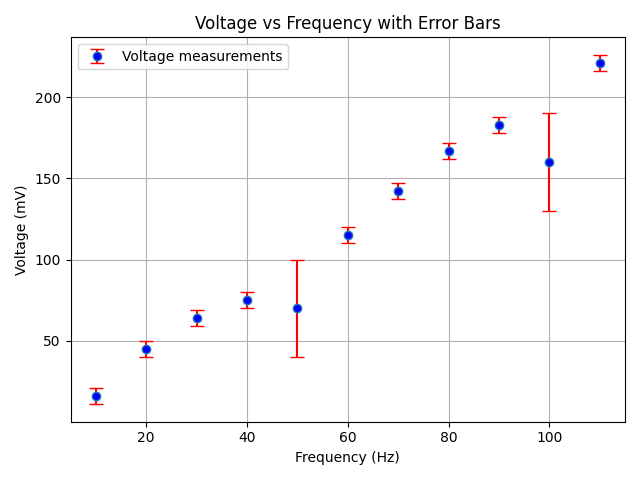
\includegraphics[width=0.95\textwidth]{./code/punto_6_1_a.png}
  \end{center}
\end{figure}

\begin{figure}
  \begin{center}
    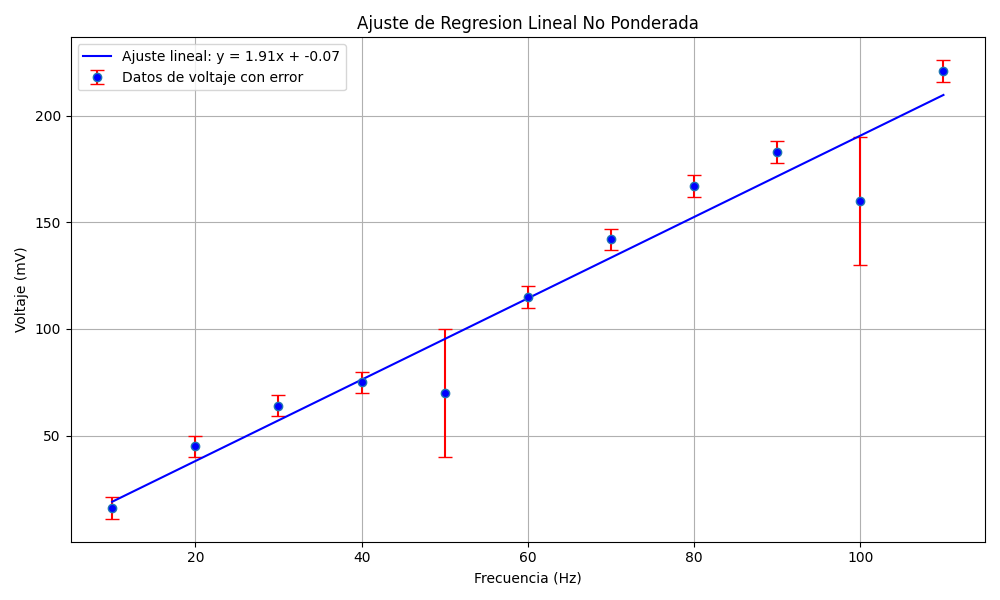
\includegraphics[width=0.95\textwidth]{./code/punto_6_1_b.png}
  \end{center}
\end{figure}


\end{document}
